\documentclass{acm_proc_article-sp}
\makeatletter
\let\@copyrightspace\relax
\makeatother

\begin{document}
% replace the name to unblind
\newcommand{\DataSeries}{DataSeries}
\newcommand{\DS}{DS}

\title{DataSeries: an efficient, flexible data format for structured serial data}
% Pretend we have one author, minimizes the space we waste on that.
\numberofauthors{1} 
\author{
\alignauthor
Eric Anderson, Martin Arlitt, Brad Morrey, Alistair Veitch  \\
 \affaddr{HP Labs. 1501 Page Mill Rd.  Palo Alto, CA} \\
 \email{\{eric.anderson4, martin.arlitt, brad.morrey, alistair.veitch\}@hp.com}
}

\maketitle
% % A category with the (minimum) three required fields
% \category{H.4}{Information Systems Applications}{Miscellaneous}
% %A category including the fourth, optional field follows...
% \category{D.2.8}{Software Engineering}{Metrics}[complexity measures, performance measures]
\category{H.3.2}{Information Storage}{}[]
 
% \terms{Structured serial data}
\terms{Design, Performance}

% \keywords{ACM proceedings, \LaTeX, text tagging} % NOT required for Proceedings
\keywords{data format, compression, performance}

{\bf TODO: Abstract}

\section{Introduction}\label{sec:intro}

Traces, recordings and measurements taken from computer systems,
networks and scientific infrastructure are vitally important for a
large variety of tasks. In every area of computer system design,
traces from existing systems have been used to validate hypotheses,
test assumptions and estimate performance. This is true of I/O
subsystems~\cite{IORef,Ji03,Uysal03}, processor
systems~\cite{ProcRef}, network systems~\cite{NetRef} and memory
systems~\cite{MemRef}, among others. Traces and logs are also
extremely useful for fault-finding, auditing and debugging purposes
~\cite{DebugRef}. Traces composed of failure data have been used to
determine system reliability~\cite{ReliabilityRef, Schroeder07,
Pinheiro07}. Trend analyses of performance information is a core
operation of various management tools~\cite{MgmtRef}. Scientific and
medical instrumentation can also generate large amounts of
data~\cite{SciRef}, which also needs to be stored, filtered and
analyzed.

The data stored in each of these diverse uses is {\it structured
serial data}, which we define as a series of records, each record
having a specified structure (i.e., containing the same set of
variables or fields). Structured serial data has four defining characteristics:
its structure is record-oriented; it is typically written only once,
and is read many times; it is usually ordered
in some manner, e.g., chronologically; and it is typically read
sequentially.  We have designed and built DataSeries, an on-disk 
data format, run-time library, and set of
tools that is optimized for storing and analyzing this type of data.
We show that the performance of DataSeries
exceeds the performance of common trace formats and databases by at
least a factor of two, and in some cases up to an order of
magnitude. DataSeries also requires far less disk space (factors vary
from 4x to 8x in test data sets).

% which we define as an ordered series of records that share a common
% structure.  This type of data commonly occurs as trace data in
% computer systems, but since the format is essentially ordered RDBMS
% tables, the need to maintain and analyze such data occurs in a large
% number of scientific fields.

There are six key properties that are desired of a data format
and analysis system for structured serial data:

\begin{enumerate}

\item \textbf{Storage efficiency}: the data should be stored in as few
bytes as possible. There are several driving factors behind this
requirement. Firstly, the amount of data stored can be large (we have
I/O traces comprising billions of records), and despite rapidly
decreasing storage prices, the cost to store data can still be
considerable, particularly when the data must be kept for long periods
of time. Secondly, we have learned that one of the primary factors
behind analysis efficiency is the speed at which data can be
retrieved. Regardless of the storage technology used, more highly
compressed data can substantially speed access times.

\item \textbf{Access efficiency}: accessing, interpreting and encoding
trace data, whether reading or writing, should make efficient use of
CPU and memory resources. From experience and experimental analysis,
we have learned that the second major factor determining analysis
efficiency is the CPU overheads of intepreting data once it has been
read off disk.

\item \textbf{Flexibility}: adding additional fields should not affect
users of the trace data.  Removing or modifying data fields should
only affect programs that use those fields and the system should
catch incorrect usage.  Further, the format should not constrain
the type of data being stored, and should allow multiple record types
in a single file. Again, experience has taught us that formats that
are not flexible lead to severe maintenance issues for both the format
interpretation code and analysis systems.

\item \textbf{Self-describing}: the data set should contain the
metadata that describes the data. This is another experience-driven
requirement, as we have had problems in trying to interpret and use
trace data from other organizations, and maintaining organizational
knowledge of our own metadata over time.

\item \textbf{(Re)Usability}: the data format should have an
associated programming interface that is both expressive and easy to
use. In particular the user model of the data and its analysis should
be easy to describe and the interface to it should easily allow for
common operations (e.g., scanning an entire data set, and processing
specific fields only).

\item \textbf{Integrity}: many structured serial data files contain
information that needs to be maintained archivally. To protect against media
errors or incorrect software systems, DataSeries files need to be
self-contained and contain internal checksums that enable
integrity checking.

\end{enumerate}

There are, inevitably, tradeoffs to be made in these requirements. For
instance, XML is an extremely flexible data format, but is not very
efficient. In the course of our work (which tends towards the analysis
of very large data sets), and the design of DataSeries, we have chosen
to prioritize efficiency over many of the other properties.

Although numerous tracing and measurement systems have been developed
over the last 20-30 years, we are not aware of any that meet all of
these requirements. We analyze some of these in our description of
related work (Section~\ref{sec:related}).

We provide four primary contributions in this paper.  First, we
introduce DataSeries, a data format and associated library, which was
specifically designed to meet the five key properties discussed above,
and relate some of the experiences that led us to make various
design decisions. 
Second, we discuss how DataSeries can support very large data sets
(e.g., hundreds of billions of records) on modest systems.  Third, we
describe how we have used DataSeries in practice to store a wide
variety of data types.  Fourth, we demonstrate the performance and
storage efficiency of DataSeries in a set of controlled experiments,
using empirical data sets. Throughout, we have tried to emphasize the
lessons learned and how they might be applied to other fields.

Since DataSeries software is publicly available (under a BSD software
license), and given the benefits of DataSeries that we demonstrate, we
argue that DataSeries should be considered for use by any application
that needs to store large amounts of structured serial data. Indeed
the Storage Networking Industry Association (SNIA) I/O traces tools
and analysis (IOTTA) technical working group~\cite{iotta-website} has
proposed DataSeries as the standard format for I/O trace data.
% and is
% currently specifying the semantics for I/O traces encoded using DataSeries.

The remainder of this paper is organized as follows.
Section~\ref{sec:related} describes the strengths and weaknesses of
existing storage technologies relative to DataSeries.
Section~\ref{sec:design} describes the design of DataSeries, including
on-disk and in-memory formats, and introduces the programming model.
Section~\ref{sec:results} presents empirical and benchmark results
from our use of DataSeries to illustrate and quantify the benefits of
DataSeries. Section~\ref{sec:conclusions} concludes the
paper with a summary of our work.
% and a list of future directions.

\section{Related work}\label{sec:related}

We classify the related work into three categories:
those that use a customized binary format, those that use a
text-based format, and relational database systems. 
For more complete comparisons including performance
results, please refer to~\cite{DSTechnicalReportSnapshot}.

Custom binary formats are usually serialized or directly written
versions of an in-memory data structure.  As such, they usually
achieve properties 1 and 2, and fail to achieve properties 3-5,
although as we will show in the results, unless the authors are
careful they can also fail to achieve property 2.

Text formats such as Column Separated Value (CSV) can
%often (but far from always)
achieve properties 3 and 4. XML achieves properties 3-5.  However,
they fail to achieve property 1, and can fail property 2 by multiple
orders of magnitude.  Even very tuned CSV
implementations can only get to within 2-7x the
access-efficiency of DataSeries, and 4-7x for the storage
efficiency.
% (See the DataSeries technical 
%report~\cite{DSTechnicalReportSnapshot} for these results.)
%{\bf TODO: need to re-do these experiments at least to
%measure the file sizes, and potentially with Tfrac text files,
%although I suspect people would use sec.usec in a block I/O trace}

Relational databases achieve properties 3, 4, and 5. RDBMS's were
designed to handle updates, so do very limited compression drastically
hurting their storage efficiency (property 1).  Our results show
$>$10x improvement on storage efficiency for DataSeries over
MySQL. 
%{\bf TODO: check the exact sizes, should be around there.}
Similarly, the generality of SQL can hurt it.  Even for fairly simple
queries running entirely on in-memory data, DataSeries runs 2-7x
faster than MySQL. 
%{\bf TODO: re-do these numbers with parallel
%decompression, etc.}  
Retrieving the data for a more complicated
calculation on the client would further slow the relative performance.

\section{Design}\label{sec:design}

DataSeries' data model is conceptually very similar to that used by
relational databases.  Logically, a DataSeries file is composed of an
ordered sequence of {\it records}, where each record is composed from
a set of {\it fields}. Each field has a {\it field-type} (e.g.,
integer, string, double, boolean) and a name. A DataSeries record is
analogous to a row in a conventional relational database. We call the
type of a row the {\it extent-type} because an {\it extent} contains a
collection of rows with the same fields and field-types. A collection
of extents is analagous to a database table.

\subsection{Data format}

A single DataSeries file comprises a collection of extents
(potentially with different extent-types), plus a header and
extent-type extent at the beginning of the file, and an index extent
and trailer at the end of the file. The header on a DataSeries file 
contains the DataSeries
file version, and check values that enable the reader to determine the
endianness encodings of the data types.  DataSeries files are always
written out using the native formats of the writing system. This 
typically minimizes byte-swapping overheads, as the architecture 
reading the files is almost always the same as the architecture reading
the files. The library transparently converts in the rare cases this
is not true, and DataSeries files can be explicitly ``repacked'' if desired. 

The extent-type extent contains records with a single string-valued
field, each of which contains an XML specification that defines the
extent-types of all the other extents in the file. We chose to use XML
to define our extent types because we saw no point in creating a new
grammar for representing this information, it is flexible (for
instance, it easily allows the addition of options describing
fields) and allows embedded comments.
% and SQL create table
% statements did not have a representation for the packing options we
% wanted to specify.

The trailer
consists of the offset and size (after compression) of the index
extent.  The offset is used to read the index extent, which has two
fields, an extent-type and an offset, to allow direct access to
extents of a single type. Storing the index and trailer at the end
of the file enable efficient writing, since writing applications will
often not know, a priori, what the final extent sizes will be, so space 
for the index cannot be allocated until after the extents have been written.

Each extent consists of a header, followed by the fixed
size data and the variable sized data.  Both fixed and variable sized
data may be compressed, using any one of a number of standard
compression algorithms~\cite{GZIP,BZIP,LZF,LZO}.  The extent header contains
metadata about the data in the extent, such as the compressed sizes of
the fixed and variable data, the number of records in the extent, the
uncompressed size of the variable length data, the compression mode,
the extent-type of the extent, and checksums of the extent before and
after compression to guard against hardware and software errors.
Checksum validation is usually disabled during extent reading to improve
performance at the cost of reduced integrity.

The extent format is designed for efficient access. Values are packed
so that once an extent is read into memory, an analysis can iterate
over the rows simply by increasing a single counter, as if for an
array containing structures.  Individual values are accessed by an
offset from that counter and a C++ cast operation. This technique
could be applicable to anyone storing similar data, e.g. RPC fields or
a streaming RDBMS.

As we initially built DataSeries prototypes, we realized the need to
add options that control various aspects of the field and extent
descriptions in order to meet the storage and access efficiency and
flexibility requirements.  While space precludes a full description
(see~\cite{DSTechnicalReportSnapshot}), we describe some of the more
significant below:


\begin{itemize}

\item \textbf{nullable fields}: there are many instances when a field
value may or may not be present, and we found it useful to be able to
indicate that a given value is null. This option is implemented by
generating a hidden boolean column that determines if the value is null.

\item \textbf{double scale}: often, the full precision of double
values is not needed. In this case, it is possible to get
significantly more compression by zeroing the pseudo-random lower
order bits by scaling and rounding. This option lets the user specify
a specific scale factor for the values stored.

\item \textbf{relative packing}: specify that a given field be packed
relative to another, using delta encoding. This option is also useful
for timestamps and index values that may be large, but are only small
relative to each other. This enables fewer bits to be used to store a
given value.

\item \textbf{unique packing}: ensures that every string (arbitrary
length binary data) field is stored only once. If a given data set
contains many repeated values, this option can significantly increase
the effective compression ratio (compression algorithms only partially
remove duplicate data).

\item \textbf{time handling}: {\bf TODO: describe experiences
and solutions here}

\end{itemize}

\subsection{Programming model}
%{\bf TODO: maybe this should be a section}
Four general functionalities are supported by DataSeries:
reading a DataSeries file, 
analyzing the data in a DataSeries file,
writing a DataSeries file,
and writing an alternative output format (e.g., CSV).
These functionalities meet all of the typical needs for
users of structured serial data, and thus facilitate
the usability (property 5) of DataSeries.

There are two key concepts in the C++ API provided by DataSeries. The
first is that of an \textit{ExtentSeries}, which is an iterator over
the rows in at least one extent.  
%When reading
%a file, the ExtentSeries is initialized with the extent, each row is
%iterated over, and then the series is reset to use the next extent.
The second key concept is that of a \textit{module}, which provides
functionality similar to the modules in River~\cite{river99}, and the
iterator model~\cite{graefeQueryProcessing93} in relational databases.
The ability to add functionality in a modular fashion enhances
the flexibility (property 3) of DataSeries.

DataSeries also provides modules that enhance the access efficiency
(property 2).
With DataSeries, each module processes an extent at a time, and
iterates over each of the rows in the extent.  In the standard
iterator model, a tree of modules are created and each module provides
a {\tt getNext()} operation that reads the next row from that module.
This model is inefficient as each row is handled as a separate data
structure.  To address this, DataSeries provides a 
bulk iterator model which amortizes the cost of reading each
row by collecting multiple rows together.  The row analysis module
used above then calls the processRow() function on each row.  For
efficiency reasons, the transfer of extents between modules is a
transfer of ownership, i.e., the module that returns an extent must
not continue to access it. We are considering relaxing this
constraint in the future to allow multiple modules to read-share a single
extent at the same time so that we can increase the available parallelism
for analysis without increasing the memory requirements.
%Each module can iterate over the rows in
%the extent by putting it into a series and using the series iterator
%to select the row and the fields to access rows in that series.
DataSeries also provides modules which exploit parallelism in operations,
such as decompressing or compressing and writing
extents to disk in parallel, which increases the access efficency
(property 2) on multi-core systems.

The DataSeries source distribution contains numerous other built-in 
general modules as well as many analysis modules, for analyzing
specific data types such as NFS, LSF and logical/physical disk volume
traces.  More detailed information on these modules and programming
examples are available 
in~\cite{DSTechnicalReportSnapshot} and the source distribution.

\section{Performance results}\label{sec:results}

%{\bf TODO: I wonder if we should rename these ``Harvard'' traces
%rather than Ellard?}
%{\bf TODO: add sections here to fill up space somewhat}
%We performed various experiments to measure the effectiveness of
%DataSeries' compression techniques, and then further compared
%DataSeries to data encoding and analysis using MySQL, CSV, CStore,
%Dan Ellard's NFS traces~\cite{ellard03}, and the 1998 World Cup Web
%traces~\cite{ita-wcweb98} for compression ratio and analysis execution speed.
%Due to space constraints we give example results from our
%comparison with Ellard and comment on highlights of our other results.

% added by Martin
In this section we provide examples to illustrate quantitatively the 
effectiveness of DataSeries.  
Section~\ref{sec:scale} describes how we have used DataSeries to store 
and analyze a large dataset on a modest system.
Section~\ref{sec:efficiency} demonstrates the flexibility provided
by DataSeries for selecting between storage and access efficiency needs.
Section~\ref{sec:ellard} provides a case study which illustrates
both the reusability of DataSeries and its access efficiency compared
to existing work.
Additional examples and comparisons can be found in the
DataSeries technical report~\cite{DSTechnicalReportSnapshot}.

\subsection{Scalability}\label{sec:scale}

The largest dataset we have is a trace of NFS traffic to and from
busy enterprise file servers.
The primary extent type 
in this data is the common records which store information about each
of the 200 billion request and reply messages. We have secondary tables that
store information about each packet captured, operations that included
file attributes, read and write requests and mount requests.  The total dataset
is about 5TB in size.

As a demonstration of the real-life performance of
DataSeries, consider the following example.  Utilizing our NFS
trace, we performed an analysis of the throughput
%effects if servers were instead accessed across a WAN.
% MFA: need to change above description of trace if we say servers
effects if the server was instead accessed across a WAN.
The analysis read in 45.5 GB of data (406 GB when uncompressed), and
processed 7.6 billion records (each record corresponds to an NFS
transaction).  Using a 2003 model two-way 2.8 GHz Xeon server, the
entire data set was processed in 11,263 wall clock seconds (about 3
hours), or roughly 675,000 rows per second while performing a set of complex
analyses.



\subsection{Examining storage and access efficiency}\label{sec:efficiency}

{\bf TODO: Jeff thinks we spend too much time on this topic. I tend to 
agree with him. Need to reduce this section, and select some other results,
and make sure they match with claims from earlier in paper about performance,
space efficiency etc. AV }

%MFA: from \subsubsection{Compression microbenchmark}

DataSeries currently supports four different compression algorithms
(bzip2~\cite{BZIP}, gzip~\cite{GZIP}, lzf~\cite{LZF} and lzo~\cite{LZO}),
and an arbitrary extent size for record data.  Empirical knowledge and
algorithm author data seem to indicate that the algorithms are
optimized for different usages.  For example, bzip2 is commonly
believed to compress better than gzip, albeit more slowly.  Also,
all compression algorithms in common use today use a compression
window, giving the impression that compression ratio and perhaps
compression and decompression rate are optimized for files above a
certain size (i.e., the window size).  
We evaluated the compression ratio, compression rate, 
and decompression rate for each of these algorithms
using various extent sizes.

Several of the compression algorithms (bzip2 and gzip)
have tunable parameters, which trade 
off compression rate for increased compression ratio.
We evaluated a range of settings for each of these algorithms.  
For the remainder of this section, we utilize bzip2 level 9 as
the representative for bzip2, and gzip level 6 as the representative
for gzip.  We found these levels provide reasonable tradeoffs
between the compression rate and ratio for each algorithm respectively.

Extent size determines the maximum window of data a compression
algorithm can look at.  For very small extent sizes, we expected to
see poor compression ratios because redundancy that would have been
within any algorithm's window size was artificially being blocked.
For very large extent sizes, we expected to see differentiation among
algorithms based on their window sizes.

The microbenchmark consisted of reading each DataSeries file
and recompressing with the compression
algorithm under study.  The uncompressed data size was divided by the CPU time for the compression
operation  to compute {\em
Compression Rate}.  Next, the same file was decompressed and its
content thrown away.  The uncompressed data size was divided by the CPU time 
to compute the {\em Decompression Rate}.  
Finally, the compressed DataSeries file size was
divided by the uncompressed DataSeries file size to determine the {\em
Compression Ratio}.  The decompression and compression operations were
performed three times for each data file in each dataset.  All microbenchmark 
measurements were taken with checksum validation enabled.

Tradeoffs exist between storage and access efficiency.  We
explore these tradeoffs, and the flexibility of DataSeries, via
several experiments.
For online creation of DataSeries files we care about the compression
rate and the compression ratio.
Figure~\ref{fig:comRateRatios} compares these metrics
with one point for each extent size.  The compression rate is shown
in log-scale because the different algorithms have vastly different rates.
This figure shows that lzf dominates
with regard to compression rate, but gzip is a good tradeoff between
compression ratio and rate, sacrificing 10x the rate to get 2x
the compression.  bzip2 is useful if very high compression
ratios are desired, while lzo is dominated by all others on this graph.
Neither bzip2 nor lzo is likely to be suitable for online file creation.


\begin{figure}[tbh]
\epsfig{width=2.5in, angle=270, file=graphs/amd/plotComRateRatio-srt.ps}
\caption{ Compression rate versus compression ratio results for disk trace data.}
\label{fig:comRateRatios}
\end{figure}

Figure~\ref{fig:decomRateRatios} compares the algorithms by the
compression ratio and decompression rate metrics.  This is important
for repeated analysis of data, a very common use case for
DataSeries.  In this case, lzo dominates the other algorithms in
terms of decompression rate (\~175 MB/s), while still keeping a
reasonable compression ratio (\~6:1). lzo is strictly superior to lzf.
bzip2 achieves 
%$2\times$
2x increase in compression ratio, but at a 
%$10\times$
10x
reduction in decompression rate.  gzip achieves negligibly higher
compression ratios at a 
%$1.3\times$ 
1.3x reduction in decompression rate.
Thus, gzip might only be considered if
lzo's compression time is too excessive or space is critical.

\begin{figure}[tbh]
\epsfig{width=2.5in, angle=270, file=graphs/amd/plotDecomRateRatio-srt.ps}
\caption{ Decompression rate versus compression ratio results for disk data.}
\label{fig:decomRateRatios}
\end{figure}

%\subsection{Ellard Traces}\label{sec:ellard}
\subsection{A case study}\label{sec:ellard}

In an effort to experiment with using DataSeries to represent and
analyze traces generated by other people, we converted the NFS
traces used by Ellard \textit{et al.}~\cite{ellard03} into DataSeries.  
The ``Ellard traces''
were originally stored as compressed text files, one record per line.
The first part of each line is a series of fixed fields, followed by a
set of key-value pairs, and finally some debugging information.  As
part of the tools, there is also a scanning program which reads the
trace files and outputs summary information for a trace.

Our evaluation came in two parts.  First, we wrote programs that
converted between the two formats.  The reversable conversion
guaranteed that we were properly preserving all of the information.
We found that the DataSeries files were on average 0.77x the size of
the original files when both were compressed using gzip.  The
compression improvements came as a result of the duplicate
elimination, the delta encoding, and the usual improvement of binary
encoding of text data.

Second, we
wrote an analysis program that implemented the first three examples in
the README that came with the tools.  We found that our analysis
program ran about 76x faster on those data files than the text
analysis program that came with the distribution.  We also found that
if we utilized lzo compression which decompresses more quickly than
gzip, our analysis program ran about 107x faster, in exchange for
slightly larger (1.14x) data files.  This also illustrates how
DataSeries can be optimized for a given purpose (e.g., greater
compression for archival storage versus faster decompression for more
efficient analysis). The detailed experimental setup can be found in
the DataSeries technical report~\cite{DSTechnicalReportSnapshot}.


 
\begin{table*}
\centering
\begin{tabular}{|r|r|r|r|r|r|r|} \hline
            & mean     & mean       & mean     & CPU     & mean     & Wall time \\
algorithm   & user (s) & system (s) & CPU (s)  & speedup & wall (s) & speedup  \\ \hline
ellard-gz   & 537.58    &  7.80     & 545.38   &  1.000x & 545.71   &   1.000x \\
ellard-bz2  & 638.48    & 12.68     & 651.16   &  0.836x & 571.49   &   0.955x \\
\hline
ds-gz-512k  &  22.91    &  3.62     &  26.53   & 20.557x &   7.16   &  76.186x \\
ds-gz-64k   &  21.45    &  1.14     &  22.59   & 24.147x &   5.81   &  93.945x \\
ds-gz-128k  &  23.30    &  1.19     &  24.49   & 22.268x &   6.30   &  86.604x \\
\hline
ds-bz2-16M  &  94.38    & 11.82     & 106.20   &  5.136x &  27.66   &  19.732x \\
\hline
ds-lzo-64k  &  18.71    &  1.14     &  19.85   & 27.472x &   5.10   & 106.897x \\
ds-lzo-128k &  21.15    &  1.10     &  22.25   & 24.514x &   5.74   &  95.022x \\
ds-lzo-512k &  24.07    &  4.07     &  28.14   & 19.382x &   7.40   &  73.762x \\ \hline
\end{tabular}

\caption{
Summary of performance results for the two analysis programs
operating on a variety of input files.  The analysis was run over the
anon-home04-011118-* files.  For the ellard {\tt nfsscan} program
the text files were compressed with either gz or bz2.  For the
DataSeries {\tt ellardanalysis} program, the DataSeries files were
compressed with either gz, bz2, or lzo, and used various extent sizes
as specified.  CPU and wall time are both relative to ellard-gz.
}

\label{tab:summary}
\end{table*}


Table~\ref{tab:summary} presents the summary results, showing the
significant speedup and reduction in CPU time that can be achieved by
using DataSeries.  The different sizes specified after the compression
algorithm for the DataSeries rows are the extent sizes. 
For example, ds-gz-512k corresponds to DataSeries with gzip
compression and a 512 KB extent size.
The substantial increase in system time for dealing
with large extents for bzip2 is a result of glibc's use of mmap/munmap
for large allocations.  Every extent results in a separate pair of
mmap/munmap calls to the kernel and hence a substantial amount of page
zeroing in the kernel.  

\subsection{Other results}\label{sec:otherresults}

We have performed a number of other experiments that demonstrate
DataSeries' benefits. Due to space considerations, we will only
describe them briefly. One study of data compression showed that for a
relatively large disk I/O trace, DataSeries provides superior disk
space utilization; stored in DataSeries, the trace consumed 1.9GB of
disk space, but 14GB in CSV format and 8.5GB as a MySQL
database. Using the same trace in a series of analyses showed that
DataSeries delivers results 6-7x faster than both formats.

\section{Lessons learned}\label{sec:lessonslearned}

{\bf TODO: this needs to become a summary section of highlights from lessons
learned. The list below are just ideas for this - all of them are discussed
in (varying) detail in the body of the paper}

Trick with cast to make data access fast: The format is designed for
efficient access. Values are packed so that once an extent is read in,
an analysis can iterate over the rows simply by increasing a single
counter, as if for an array of a structure.  Individual values are
accessed by an offset from that counter and a C++ cast.  applicable to
anyone storing similar data (RPC, streaming DB...)

Delta encoding via the pack\_relative field option saves space
sometimes a lot, with x cost.

Unique packing saves strings only once, improving on runlength
compression by having effectively an infinite window size for specific
strings.

Parallel compression and decompression improves performance
dramatically on multicore machines as evidenced by the ellard
comparison.

Bulk processing of extents amortizes compression and decompression
costs over a fixed configurable amount of space.

Byte swapping if necessary is automatically performed.

{\bf TODO: This point and the next one (about time values) are not
currently covered in the main text}. 

Making data analyses type specific improves performance greatly.
Consider the analyses of NFS data.  When new accessors were added that
did not support nullable fields, performance improved by x amount.
Compared to SQL, and dsstatgroupby type specific performance can be as
much as x faster.  However, writing type specific accessors is more
time consuming, so for one shot analyses it may not be worth the
effort.

Discuss time field issues and why the field base value was a bad idea
and where we are with archival time representation and functional time
representation now.

field base value: applicable only to double fields,
this was used to gain precision for double values. This extra degree
of flexibility was introduced when we realized that storing nanosecond
precision time values, using the unix epoch (00:00:00 UTC on January
1, 1970), was not possible with a single double. Using this option, it
is possible to specific a base value that indicates the time the
events in the data file start, and the value stored indicates the time
in nanoseconds since.



\section{Conclusions}\label{sec:conclusions}

{\bf TODO: need to incorporate lessons learned into conclusions}

We have described DataSeries, a data format that enables the efficient
and flexible storage of structured serial data. This type of data is
used in numerous applications in all areas of computing and
science. We have identified the properties required for a system that
processes such data, and shown through a series of experiements and
comparisons to other systems that DataSeries meets satisfies these
properties. In particular, DataSeries offers significant performance
and storage efficiency benefits.  
% For these reasons, DataSeries is the
% recommended trace for the SNIA IOTTA technical working group.

\bibliographystyle{abbrv}
{\small
\bibliography{tr-references}
}
% You must have a proper ".bib" file
%  and remember to run:
% latex bibtex latex latex
% to resolve all references
%
% ACM needs 'a single self-contained file'!
%
\balancecolumns

\end{document}
